\section{Elektriskt fält}
\textbf{HAREC a.\ref{HAREC.a.1.3}\label{myHAREC.a.1.3}}
\label{elektriskafält}
\index{elektriska fält}

\subsection{Potential}
\index{elektrisk potential}

Potentialskillnaden -- spänningen -- mellan olika laddade kroppar, skapar krafter
mellan varandra samt mellan dem och deras omgivning. Detta fenomen kallas
elektriskt kraftfält och är orsaken till att elektriskt laddade kroppar kan
komma i rörelse.

\subsection{Elektrisk laddning}
\index{elektrisk laddning}
\index{symbol!\(e\) elementarladdning}
\index{symbol!\(Q\) laddning}
\index{Coulomb (C)}
\index{enheter!Coulomb (C)}

Elektriska laddningar är grunden för elektricitetsläran. Varje proton i
atomkärnan är bärare av en positiv laddning. Neutronerna i atomkärnan är
elektriskt neutrala. Antalet protoner i kärnan bestämmer därför ensamt kärnans
totala positiva laddning, kallat för kärnladdningstalet. Elektronerna som
kretsar omkring atomkärnan är bärare av var sin negativa laddning.

Elementarladdningen [ e ] är den laddning som finns i en elektron och har länge
ansetts vara den minsta möjliga laddningen. Nutida elektronfysik konstaterar
ännu mindre enheter, men det går vi inte in på här.

Antalet protoner och elektroner i en atom är lika och elektronernas samlade
negativa laddning blir då lika stor som protonernas samlade positiva laddning.
När laddningar med olika polaritet är lika stora väger de ut varandra och blir
elektriskt neutrala till sin omgivning.

\begin{quote}\emph{
Måttenheten för elektrisk laddning är \(Coulomb\ [C]\).
}\end{quote}

Laddningsmängden \(1\ Coulomb\) motsvarar 6,25 triljoner (\(6,25\cdot10^{18}\))
elementarladdningar.

Sambandet mellan laddning och ström är

\begin{quote}
\(Q = I \cdot t\)
\end{quote}

Laddning [Q] är ström [I] under tiden [t]

\begin{quote}
\(1\ C = 1\ A \cdot 1\ s = 1\ amperesekund\ [1\ As]\)

\(1\ Coulomb = 1\ Ampere \cdot 1\ sekund\)
\end{quote}

\subsection{Kraftfält omkring elektriska laddningar}

\begin{figure}
\begin{center}
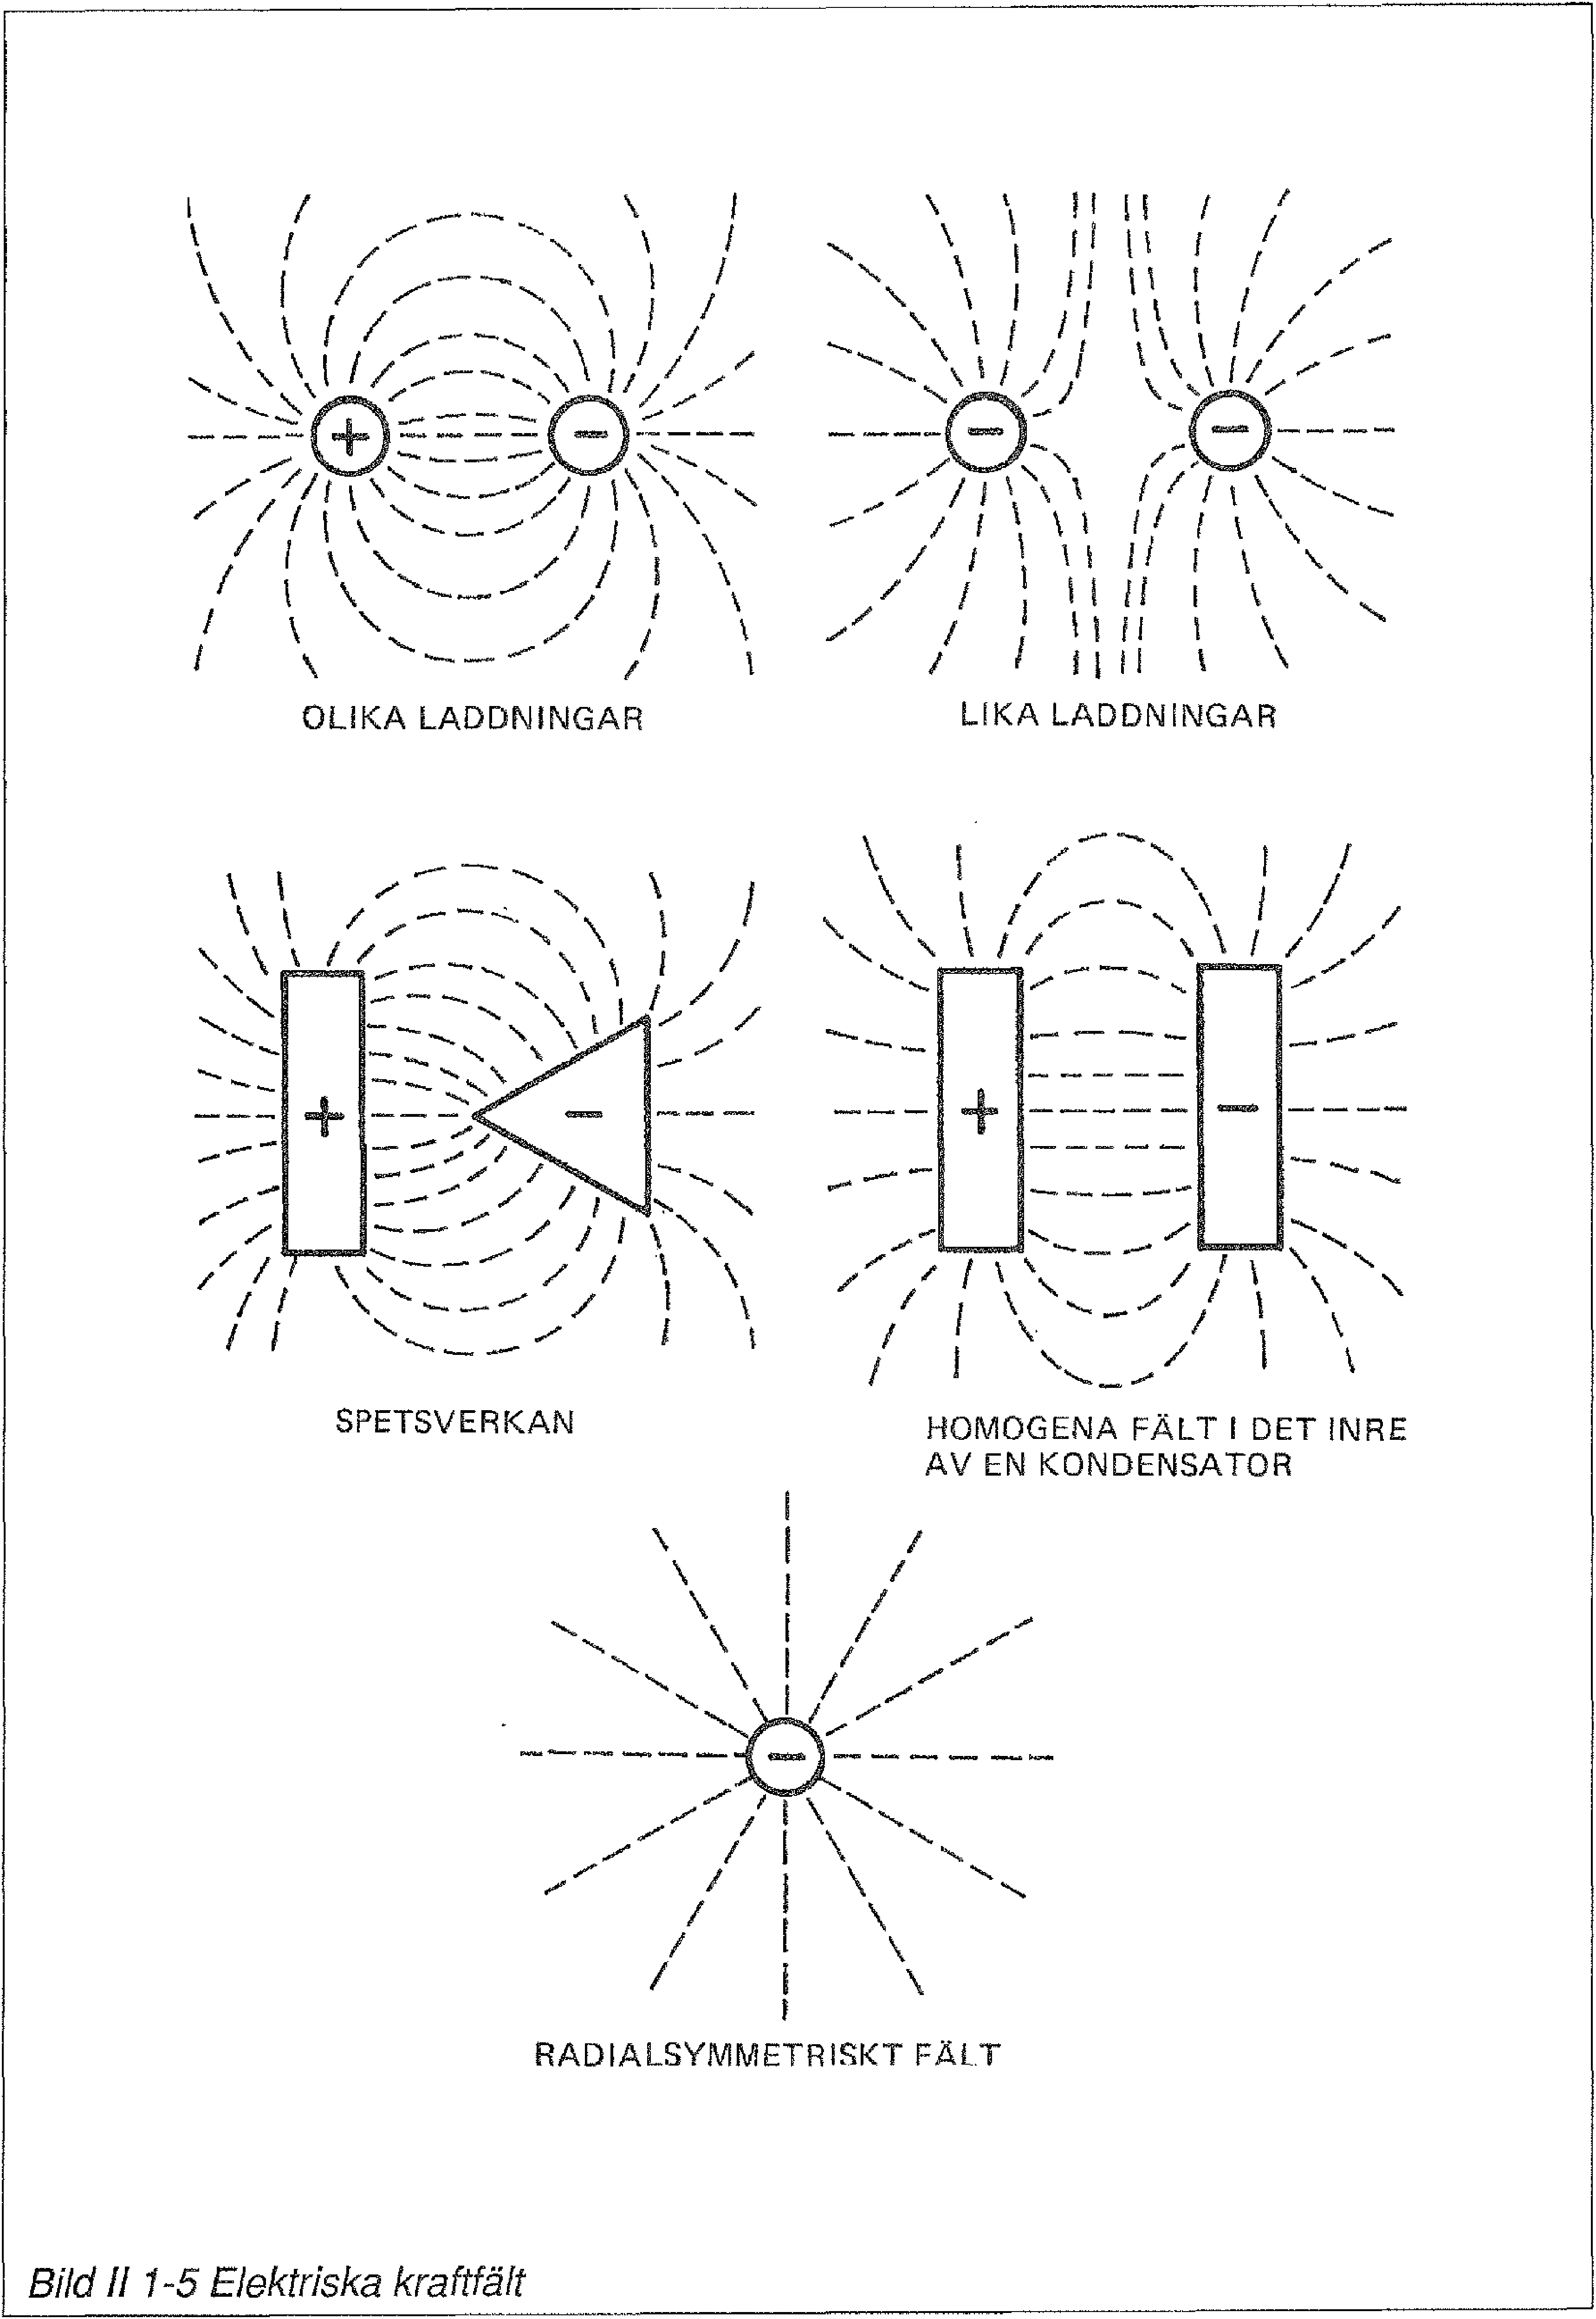
\includegraphics[width=\textwidth]{images/bild_2_1-05}
\caption{Elektriska kraftfält}
\label{fig:BildII1-5}
\end{center}
\end{figure}

Fig. \ref{fig:BildII1-5}

Mellan elektriska laddningar bildas krafter.

\begin{itemize}
\item Varje laddning är omgiven av ett elektriskt kraftfält.
\item Mellan positiva (+) elektriska laddningar
och (-) negativa laddningar bildas krafter.
\item Fältkrafternas styrka och riktning symboliseras som linjer mellan positiva och
negativa laddningar, där styrkan är densamma utmed respektive linje.
\end{itemize}

(även 1.1)

\begin{quote}
\emph{Kroppar med olika slags laddningar dras till varandra}

\emph{Kroppar med lika slags laddningar stöter bort varandra}

\emph{Oladdade kroppar påverkas inte och ger ingen kraftverkan.}
\end{quote}

\subsection{Elektrisk fältstyrka}
\textbf{HAREC a.\ref{HAREC.a.1.3.1}, a.\ref{HAREC.a.1.3.2}\label{myHAREC.a.1.3.1}\label{myHAREC.a.1.3.2}}
\index{elektrisk fältstyrka}
\index{symbol!\(E\) elektrisk fältstyrka}

\begin{wrapfigure}{R}{0.5\textwidth}
  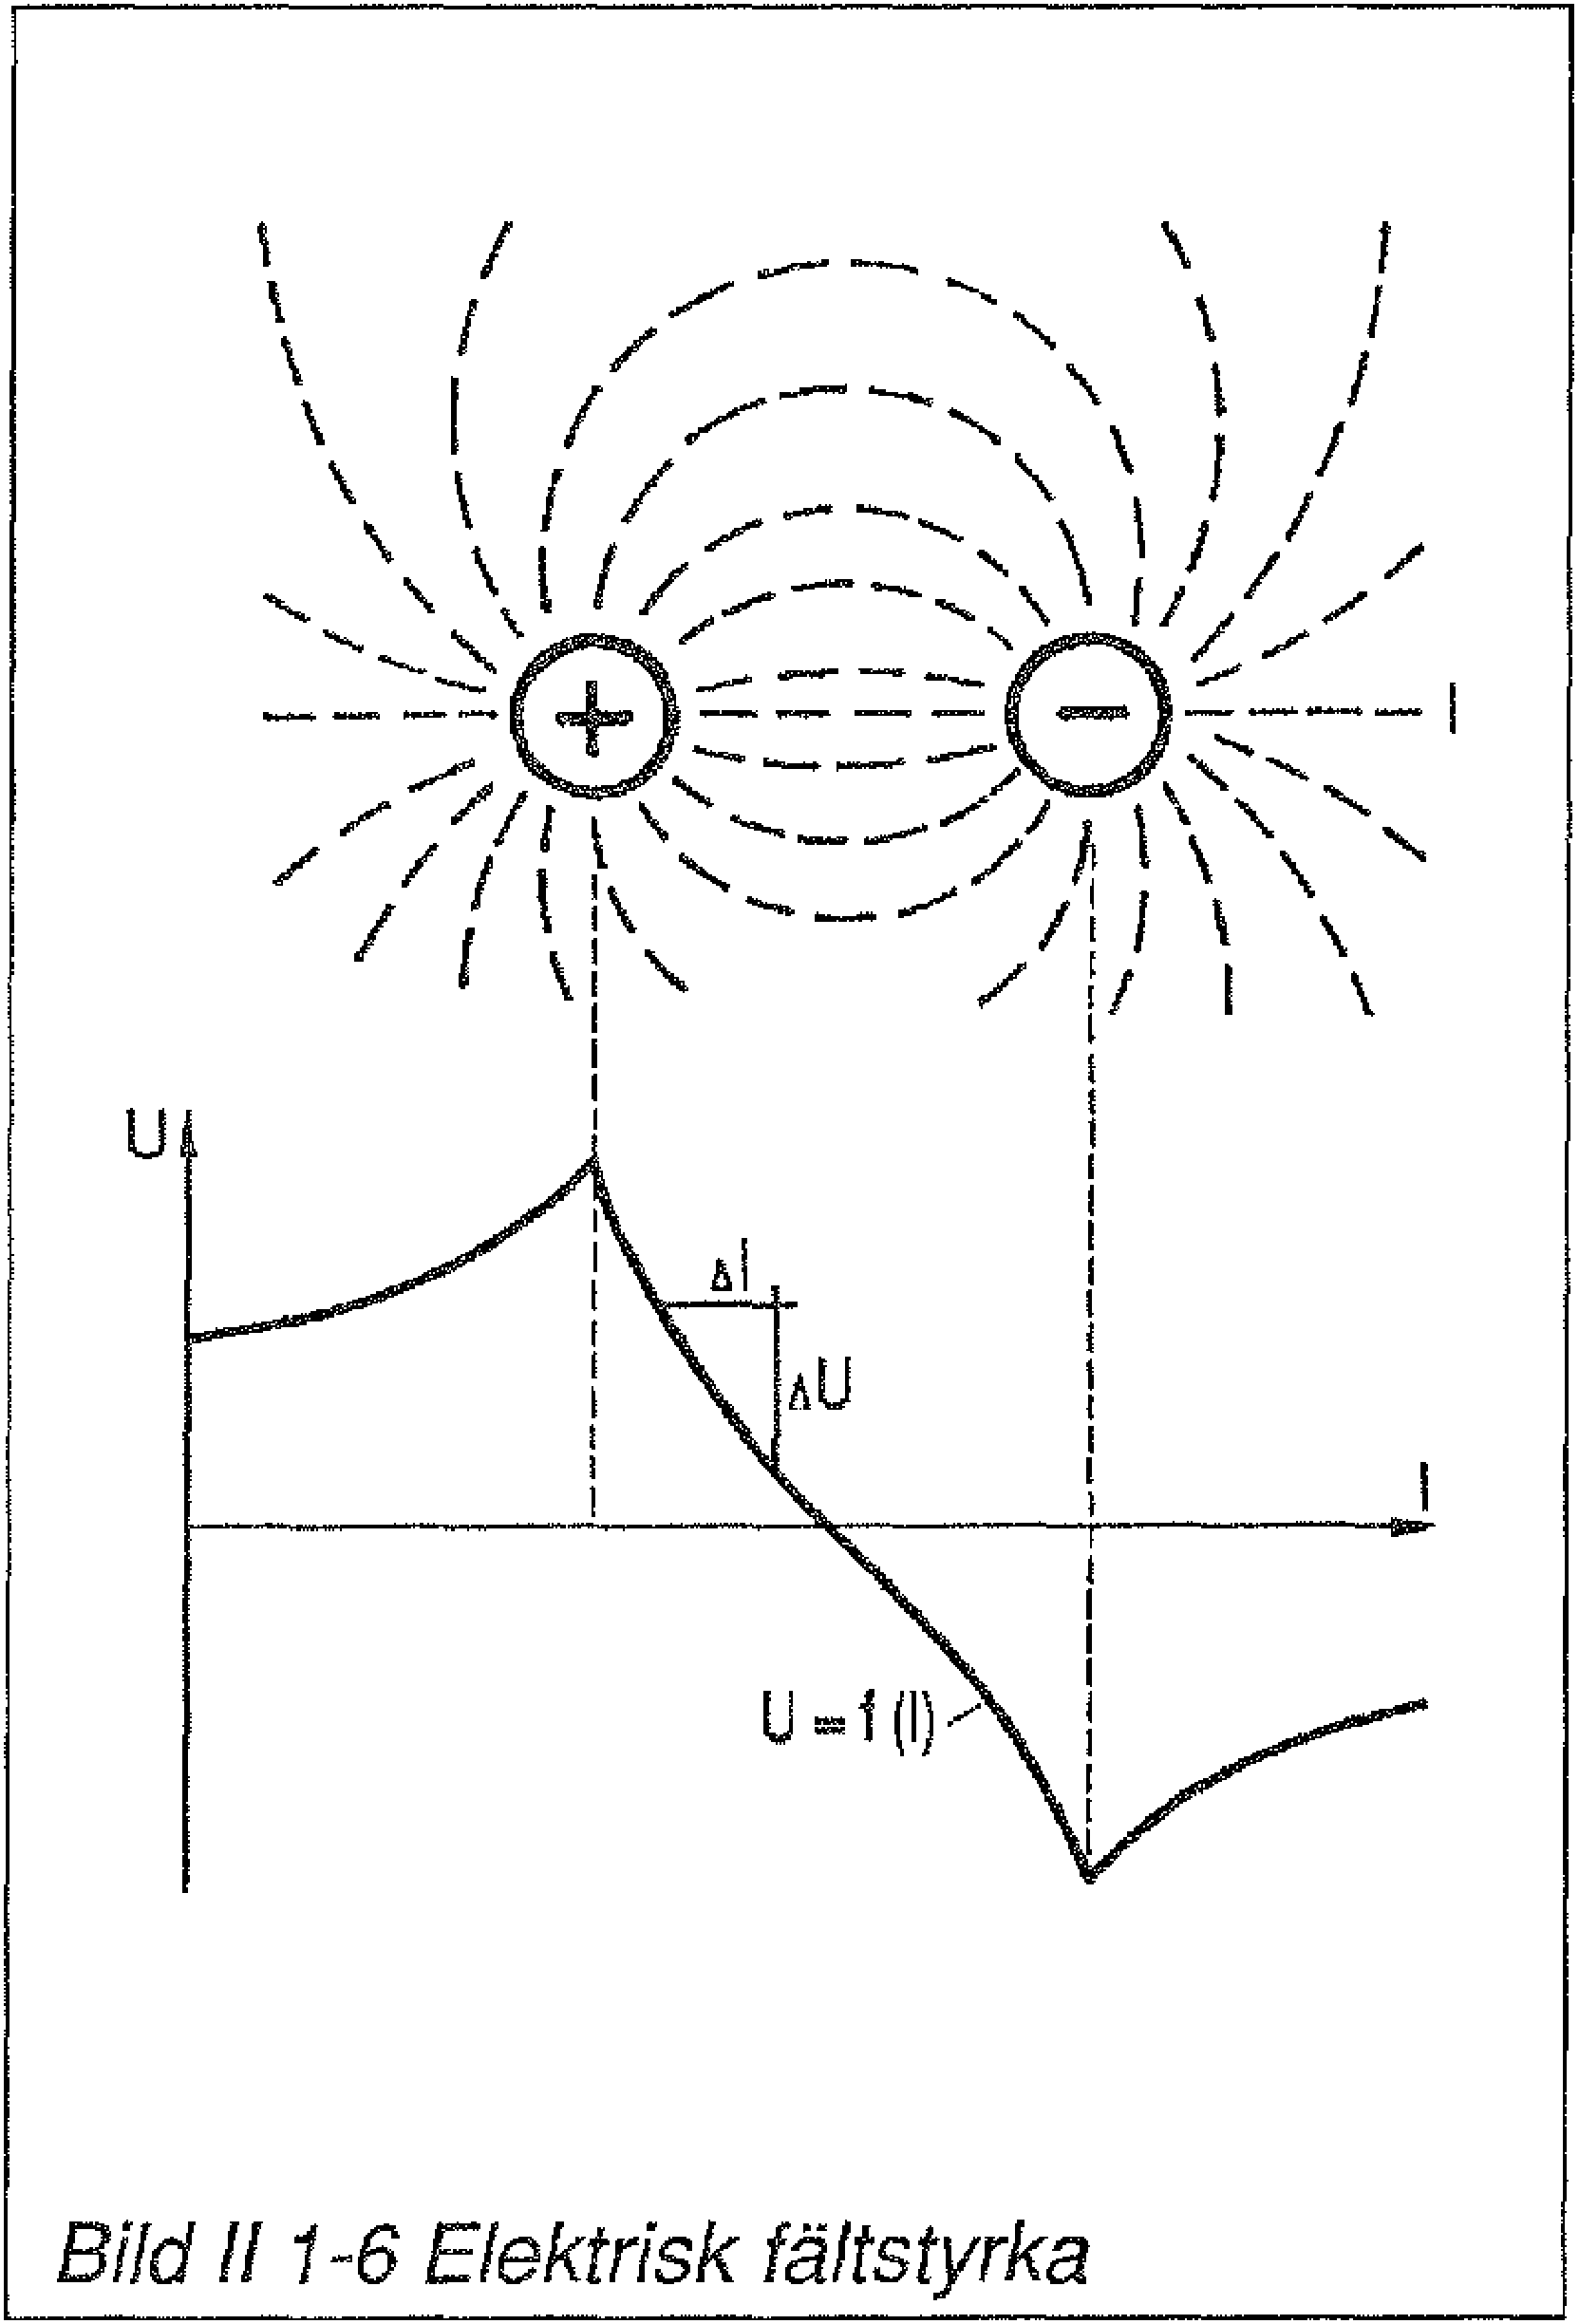
\includegraphics[width=0.5\textwidth]{images/bild_2_1-06}
  \caption{Elektrisk fältstyrka}
  \label{fig:BildII1-6}
%  \vspace{-30pt}
\end{wrapfigure}

I en trådformad ledare, som det flyter likström igenom, fördelas strömmen lika
över tvärsnittet. Om ledaren i stället är ett tunt plan, så blir
strömfördelningen annorlunda. Bilden visar ett plan med två elektroder, som
anslutits till en spänningskälla. Utmed sträckan mellan elektroderna fördelas
strömmen över planet så som strömlinjerna på bilden. Fördelningen beror på
elektrodernas utformning och polaritet. Strömtätheten är inte lika över hela
planet, eftersom planet kan ses som många parallellkopplade resistorer vars
resistanser ökar med tilltagande strömlinjelängd.

Strömtätheten i planet är större där resistansen mellan elektroderna är liten.
Närmast elektroderna där alla strömlinjer samlas är strömtätheten extremt hög.
Där strömtätheten är som störst finns den största potentialskillnaden
(spänningen) per längdenhet strömlinje. Man kan mäta potentialerna i planet.
Spänningen mellan två punkter utmed en tänkt strömlinje är därvid proportionell
med linjens längd mellan punkterna. Halva spänningen finner man mitt emellan
punkterna.

Elektriska fält är upplagrad energi. Fältstyrkan kan bli så hög, att det blir
en urladdning mellan polerna. Korona från ändarna av en antenn är ett annat
tecken på hög fältstyrka. För att försvåra urladdning kan man öka elektrodytan,
t.ex. göra den klotformad. Omvänt kan man medverka till urladdning genom att
minska elektrodytan. Ett exempel är åskledarens spets.

Fig. \ref{fig:BildII1-6}

I diagrammet \(U = f(l)\) visas spänningarna utmed ''mittströmslinjen'' I genom
plus- och minuspolerna. Kurvutseendet är typisk även för omkring liggande
linjer, oavsett längd.

Bilden framställer en ledare som ett idealt plan, medan den i praktiken är en
volym. För att efterlikna en volym föreställer vi oss att bilden roterar
omkring mittströmslinjen, med fältlinjerna oförändrade. Även om resistansen i
den rotationskropp som uppstår är så hög att ingen ström flyter, så är
spänningsbilden fortfarande densamma.

Spänningsbilden gäller även för isolerande fasta material, gaser och vakuum.
Det finns alltså spänning mellan olika punkter även i ''friska luften''. Denna
spänningfältstyrka- kan mätas med särskilda instrument, s.k. fältstyrkemätare.

Av brantheten på spänningskurvan i bilden framgår vilken delspänningen är per
dellängd av en spänningslinje. Kvoten av delspänning och avståndet mellan
mätpunkterna kallar man för elektrisk fältstyrka.

\begin{quote}
\emph{I formler betecknas elektrisk fältstyrka med bokstaven \(E\).}
\emph{Elektrisk fältstyrka mäts i volt per meter.}
\end{quote}

\(
\begin{array}{cc}
E=\dfrac{\Delta U}{\Delta l} & \dfrac{[volt]}{[meter]}
\end{array}
\)

\subsection{Skärmning av elektriska fält}
\textbf{HAREC a.\ref{HAREC.a.1.3.3}\label{myHAREC.a.1.3.3}}
\index{elektriska fält!skärmning}
\label{elektrostatik skärmning}

I grunden finns det två slags fält, det elektriska och det magnetiska. Dessutom
finns det även elektromagnetiska fält, som är sammansatt av båda dessa. Fält
kan vara statiska eller dynamiska, varav här avses dynamiska. Ett dynamiskt
elektriskt fält genererar ett magnetiskt fält. Omvänt generar ett dynamiskt
magnetiskt fält ett dynamiskt elektriskt fält. Denna växelverkan gör att fälten
kan hållas igång av varandra med tillskott av yttre energi.

Fält i rörelse alstrar elektromagnetisk strålning, som påverkar omgivningen. När
påverkan inte är önskvärd måste fältet skärmas av. Ett sätt att skärma av ett
elektriskt fält är en metallisk kapsling som anslutits till apparatens
jordreferens. Skärmen behöver inte vara tät, men utförd så att all magnetiskt
inducerad ström i den bryts. (Jfr \ref{elektromagnetisk skärmning})
